\chapter{相关工作}

\section{数据驱动的交通预测}

交通流预测是智能交通系统的重要支撑技术，对城市计算、数据科学有重要的研究意义。主要目的就是利用历史的交通流量数据以及路网拓扑结构，建立可以准确反映未来某个时间段交通动态特征的预测模型，从而为交通管理优化、出行服务智能化决策提供支持。本节依照技术的发展脉络，由传统的统计学方法慢慢转向时空序列建模和深度学习范式的转变，联系学术前沿成果，着重剖析城市计算视角下大数据推动的创新应用实例。

传统的交通流量预测大多用时间序列分析和统计学习的方法来开展。自回归积分移动平均模型（ARIMA）以及它的季节性版本（SARIMA）由于具有较好的性能而被广泛应用于实际中。早在2003年，Williams和Hoel就对ARIMA模型在交通流预测中所起的作用进行了详细的分析，通过解析历史数据的时间序列特性来推断出未来的变化趋势，并建立了一个完整的建模体系\upcite{ref75_williams2003arima}。支持向量回归（SVR）、随机森林等机器学习方法也被用来加入到预测模型当中，这些方法不再需要假设数据服从某种参数化分布，可以自动从历史数据中学习出输入与输出之间的映射关系。但是这些方法的共同缺点是每次只能处理一个路段或者一个检测点的数据，不能利用路网中相邻路段之间的空间相关性 \upcite{ref6_li2018urban}。随着深度学习技术的发展，研究者也开始使用循环神经网络（RNN）、长短期记忆网络（LSTM）等模型来建模交通流的时间序列特征。Ma等人2015年最早将LSTM应用到交通速度预测中，利用门控机制克服了长序列训练中梯度消失的问题，在短时交通预测方面比ARIMA更好 \upcite{ref58_ma2015lstm}。但是时间序列模型只考虑了时间维度，没有考虑路网的空间拓扑结构。近年来的研究表明，时序预测模型在面对新的数据分布时的泛化能力也存在问题 \upcite{ref76_tao2026time}。

为了把时间序列特性同时空分布特性结合起来，学术研究领域出现了对于时空复合数据进行深度学习建模的热潮。根据模型构建原理的不同，目前的研究成果可以分为三类，分别是基于RNN的方法、基于GNN的方法和GNN与RNN融合的方法。

以循环神经网络(RNN)、长短期记忆网络(LSTM)等为代表性的建模框架，主要研究交通流量序列动态变化的特征，用融合的方式提高空间信息表达的能力。早在2015年，Ma等人就将LSTM应用到交通流速预测的任务上，通过对历史周期内速度数据序列的学习和解析，可以得到对未来趋势的准确预测。该方法对于传统递归神经网络长期依赖问题造成的梯度消失或者爆炸现象有很好的性能\upcite{ref58_ma2015lstm}。但是纯RNN方法的缺点就是它们本质上都是时间序列模型，对路网的空间结构，也就是路段之间拓扑关系以及相互影响没有直接的建模能力。虽然可以将多个路段的序列拼接成高维输入来间接引入空间信息，但是并没有考虑到路网真实的图结构。

第二类研究方法主要依托图神经网络（Graph Neural Network，GNN）框架展开。由于城市路网结构具有典型的图论性质，交叉口是节点，路段是边的关联形式给基于GNN的深入分析创造了有利条件。STGCN属于一种典型的模型，在时空数据融合方面具有明显的优势。该模型把空间卷积同时间序列处理结合起来，既较好地把握了道路网络拓扑特性，又准确地表现了交通流随时间动态改变的趋势，而且把两者有机地结合起来，创建出一个可以全面体现时空交互特点的综合分析框架 \upcite{ref7_yu2018stgcn}。Graph WaveNet提出了自适应邻接矩阵和扩张因果卷积，让模型能够自行学习节点之间的隐含空间依赖关系，而不需要预先定义完整的路网邻接矩阵 \upcite{ref9_wu2019graphwavenet}。STSGCN则设计了同步时空卷积模块，在同一层中同时处理空间邻域和时间邻域的信息，避免了传统方法中空间和时间模块分离的问题 \upcite{ref10_song2020stsgcn}。除了同步建模外，另一个研究方向是将注意力机制与图卷积结合，让模型动态地为不同的时间步和空间邻域分配权重，进一步提升时空建模的精度 \upcite{ref59_zou2024atstgcn, ref60_yao2025taidgcn}。

第三类研究范式把图神经网络(GNN)和循环神经网络(RNN)结合起来，试图对时空异质数据的深层特征进行系统的分析。其中，DCRNN（Diffusion Convolutional Recurrent Neural Network）作为这一领域的核心模型，依托扩散理论模拟交通流在路网中的传递机理。为了克服传统图卷积不能很好地建模空间关联性的问题，DCRNN引入了双向扩散卷积，大大增强了空间拓扑信息的表达能力，用门控机制优化GRU结构，在时序序列中动态维护节点的隐状态更新，用编码器-解码器架构提取长程依赖属性 \upcite{ref8_li2018dcrnn}。DCRNN训练采用计划采样（Scheduled Sampling），消除训练阶段与推理阶段分布不一致的问题。GNN编码空间依赖、RNN编码时间依赖的架构给之后的时空融合模型提供基本的设计范式。

基于上述三种方法，本研究进一步整合了注意力机制。采用ASTGCN模型时，在时空维度上引入注意力模块，使其能够在预测过程中具备动态聚焦关键道路路段与核心时间序列节点的能力，从而增强模型的适应性与精确性 \upcite{ref11_guo2019astgcn}。GMAN使用编码器-解码器配合多头注意力来显式建模长期时间依赖 \upcite{ref12_zheng2020gman}。PDFormer则进一步考虑了交通拥堵在路网中的传播延迟现象——拥堵从上游路段传播到下游路段需要一定的时间，而不是瞬间完成的。它通过设计动态长距离注意力机制，让模型能够捕捉不同路段之间带有传播延迟的远距离依赖关系，在多个公开数据集上取得了比之前的模型更好的预测精度 \upcite{ref13_jiang2023pdformer}。

作为与预测建模并驾齐驱的新兴研究方向，城市计算致力于借助多元传感技术和多源数据（含交通流量、环境监测、POI分布及社交媒体内容等）的综合分析，探究城市运作机理，并为城市治理决策提供科学依据。早在2014年，Zheng等学者便已构建了城市计算的概念框架及其理论体系与演进路线图\upcite{ref2_zheng2014urban}，明确了数据采集、数据管理、数据分析和知识发现四个层次的研究问题。在交通领域，轨迹数据挖掘是城市计算中最活跃的方向之一。通过分析大规模车辆GPS轨迹，研究者可以从中发现城市道路的通行模式、识别常发拥堵路段和时段，以及理解不同区域之间的通勤流量和方向 \upcite{ref15_zheng2015trajectory}。Yuan等人利用出租车轨迹和POI数据识别城市不同区域的功能类型，揭示了出行模式和城市功能之间的内在关联 \upcite{ref16_yuan2012discovering}。这些分析结果可以被进一步用于交通规划、信号配时优化和出行信息服务。

随着交通预测研究的深入，不同模型之间的比较和复现变得越来越困难——每个模型使用的数据集、预处理方式和评估指标都不完全一致。为了解决这个问题，研究者开发了标准化的评测框架。LibCity是其中最具代表性的工作之一 \upcite{ref61_wang2021libcity}。LibCity提供了一个统一的交通预测算法评测平台，集成了包括STGCN、DCRNN、ASTGCN和PDFormer在内的数十种主流预测模型，并在多个公开数据集上提供了标准化的数据预处理、模型训练和评估流程。BIGCity则在此基础上进一步，提出了一个通用的时空数据模型，能够统一处理轨迹数据和交通状态数据两种不同类型的时空数据 \upcite{ref62_yu2025bigcity}。

尽管上述方法在常规场景下表现良好，但它们在几个方面仍存在明显的不足。首先，这些模型主要依赖历史数值数据来做预测，无法理解视频画面、文本报告等非结构化信息 \upcite{ref63_JSJYGG202118006}，当遇到突发事件（如交通事故、临时管制的公告）时，模型没有办法把这些信息纳入预测过程 \upcite{ref64_li2024trafficanomaly}。其次，现有模型缺乏语义理解和逻辑推理的能力，用户如果需要交互式地分析交通状况，仍然需要通过编程或图形界面手动操作不同的系统和工具。近年来的时序基础模型研究尝试用大规模预训练解决通用时序预测问题 \upcite{ref65_liang2024timeseries}，但在交通领域，数据分布受路网结构和事件影响波动较大，通用的预训练策略仍然面临着迁移效果不稳定的挑战 \upcite{ref66_wang2025congestion}。这些问题的存在，促使研究者思考如何在大语言模型的基础上构建更加智能的交通分析系统。下面将介绍大语言模型工具调用和智能体技术的发展现状。

\section{大模型工具调用与智能体}

早期的大语言模型主要致力于文本生成任务的研究，其核心功能局限于接收输入并输出相应内容，难以实现与外部环境的有效交互。学术界对此类局限性给予了充分关注，并积极探索将大模型嵌入外部工具链的技术路径，以突破其固有限制并扩展应用领域。从技术层面分析，目前主流的大语言模型整合方案可归纳为三种典型模式。

该方法依靠提示词驱动技术来完成，它的主要优点就是不需要对模型内部参数进行修改，而是通过对提示词的精心设计来确定外部工具的功能定位、输入输出规范和关键参数的配置，从而引导模型在一定的场景中完成指定的外部调用任务。ReAct模型的运行过程具有循环迭代的特点，它先对当前的环境状况和目标要求进行解析，然后确定出需要的核心数据以及相应的工具调用指令，之后根据外部系统返回的结果来更新知识库，从而给接下来的决策提供支持，并且不断改进推理性能。这就实现了信息采集与智能决策的有机融合 \upcite{ref36_yao2023react}。该方法的优点在于灵活，不需要额外的训练，但是模型对于工具的理解完全依靠提示词的质量，在复杂的场景中很容易出现格式错误或者调用策略不合理的情况。

第二类就是微调法。该类方法是在训练数据里加上工具API描述及调用示例，使模型从数据中学会使用工具的方法。Toolformer最早提出这种自监督的训练范式，将特殊的调用标记插入到文本当中，使得模型能够预测出哪些位置需要用到工具，从而学会使用日历、计算器、搜索引擎等基本的API \upcite{ref32_schick2023toolformer}。ToolLLM则将这个思路扩展到超过16000个真实的RESTful API上，并设计了基于深度优先搜索的决策树算法来评估多步调用的策略 \upcite{ref34_qin2024toolllm}。微调方法的优势是模型对于工具的理解更稳定，但是缺点是要建立高质量的训练数据，每次添加一个新的工具都要重新微调。

第三类为原生支持方法。以GPT-4为代表的商用大模型把函数调用（Function Calling）作为API的原生功能提供，开发者只需要在API请求中用JSON Schema的形式定义函数的名称、参数和描述，模型就可以在对话中自动判断什么时候触发调用并返回符合格式的调用请求。Berkeley Function Calling Leaderboard（BFCL）的建立推动了这方面的评测标准化，系统性地测试了模型在单工具调用、多工具选择和并行调用等多种场景下的表现 \upcite{ref35_patil2025bfcl}。

工具调用能力的形成给智能体系统的创建打下了基础。目前以大模型为基础的智能体结构主要有单智能体和多智能体两种模式。单智能体架构是以一个大模型为中心，依靠外部工具以及记忆模块来实现用户所要求的任务。ReAct范式是单智能体典型的实现，模型
在推理、行动、观察的循环中不断进行直到任务完成。Plan-and-Execute是另一种常见的范式，它把任务分成两部分，一部分是由规划模块来生成完整的执行计划，另一部分则是由执行模块来按照这个计划依次调用工具，这种方式在处理步骤清楚的任务时效率更高，但是缺少了动态调整的灵活性。Auto-GPT和BabyAGI属于单智能体架构的早期代表应用，可以体现模型自主拆解目标、循环执行任务并且在失败时自我调节的特点。Voyager把这种思想运用到具身智能体的场景里，智能体在《我的世界》中通过自主探索来获得技能，把学到的操作保存到技能库中供以后使用 \upcite{ref46_wang2023voyager}。

多智能体架构把任务分配给不同的智能体，利用智能体之间的合作来完成任务。MetaGPT模拟出软件公司多角色分工，把产品经理、架构师、工程师、测试员等角色分别交给不同的大模型实例去扮演，这些大模型实例之间通过消息传递的方式一起完成软件开发的过程 \upcite{ref47_hong2024metagpt}。AutoGen提供了一个灵活的多智能体对话框架，开发者可以定义不同类型的智能体（如用户代理、助手代理、工具代理）并将它们组合成工作流 \upcite{ref48_wu2024autogen}。Park等人提出的生成式智能体更加重视社会行为的模拟，他们创建了25个有记忆、反思和日常计划的虚拟角色，在沙盒环境里表现出类似人类的社会互动行为 \upcite{ref49_park2023generative}。多智能体架构的优势是能用不同的模型来处理各种各样的子任务，但是系统复杂度高，智能体之间通信、协调的成本也要考虑进去。

在工具使用以及智能体落地的过程中还存在着一些关键问题没有得到完全的解决。首先就是工具调用的可靠性问题。模型在复杂的任务中，工具调用会出现格式错误、参数遗漏、调用顺序错乱等状况，在需要多步调用的时候，每一个步骤的误差都会被累积放大。其次，长任务的稳定性、效率也成问题，模型长时间运行的时候就会出现上下文超限、决策偏离初衷、进入重复循环等状况。除此之外领域知识匮乏也是普遍存在的。通用大模型对于交通等领域的知识覆盖不足，很容易给出不符合实际情况的建议，这也是目前检索增强生成（RAG）被广泛研究和应用的主要原因。下面给出智能体在各个领域具体的使用情况。

\section{智能体的应用}

近年来，基于大模型的智能体在多个领域展现出了实用价值。

在代码开发领域，智能体的应用最为成熟。OpenAI在2021年提出了Codex模型，在GitHub公开代码库上对GPT模型进行微调，使其具备了从自然语言描述中生成Python代码的能力 \upcite{ref67_chen2021codex}。基于Codex的GitHub Copilot上线之后迅速得到了大量的用户，它可以为开发者在编写代码的时候提供实时的补全建议，支持的编程语言有几十种。Claude Code和Cursor等工具又把代码智能体的能力范围拓宽了，它们不再只是对单行代码进行补全，还可以对整个代码仓库的结构有了解，可以进行跨文件的重构，自动修复编译错误，并且在多次对话之后还能完成从需求分析到代码部署的全部开发过程。这些工具本质就是一种以代码理解、生成为主的任务型智能体，它接受自然语言描述的开发需求，分析现有的代码结构来规划实现方案，调用代码编辑器的API来执行具体的修改操作。

数学推理领域里智能体也有了重大进展。传统的定理证明要数学家手动构造每一步推理的证明步骤，过程非常耗时而且容易出错。Lean等交互式定理证明工具用形式化的语言把数学证明变成可以被计算机逐行验证的代码。研究者开始尝试使用大语言模型和Lean相结合的方式来产生证明代码。2024年Google DeepMind提出AlphaProof系统，在当年的国际数学奥林匹克竞赛（IMO）中解出6道题中的4道，获得银牌级别成绩 \upcite{ref68_deepmind2025alphaproof}。AlphaProof的主要思想就是把预训练的语言模型和AlphaZero强化学习相结合，使系统在Lean的形式化环境下不断尝试生成和验证证明策略，通过自我博弈来不断提高证明的能力。这项工作证明智能体可以对高度抽象的符号推理做出贡献。大模型对于数学的定理证明有着诸多的进展，不过它所做出的答案，并不是绝对正确。思维树（Tree-of-Thoughts，ToT）方法扩展了传统的链式思维，使模型可以同时探索多条推理路径，并对这些路径进行评价和剪枝，在逻辑推理、数学应用等方面比链式思维有更好的效果 \upcite{ref69_yao2023tot}。

智能体开始参与到科学研究当中去，开始做一些文献检索、实验设计、数据分析等工作。基于大模型的科学助手可以从中提取出关键的信息并总结出研究的趋势，从而让研究人员对某一领域的发展状况有大概的了解。Sakana AI在2024年提出AI Scientist系统，实现了科研工作流的自动化，即由大语言模型自行完成提出研究假设、设计实验方案、编写和运行代码、分析实验结果、撰写完整的学术论文等所有科研工作 \upcite{ref70_lu2024aiscientist}。在机器学习的实验验证中，AI科学家生成的论文在某些指标上已经超过了顶级学术会议的接收标准。除此之外，智能体也被用来进行蛋白质结构预测、新材料筛选、药物分子设计等有明确优化目标的科学问题研究，在这些场景下，智能体可以自动生成候选方案，调用仿真工具验证方案的效果，根据验证结果不断优化，大大缩短了科研探索的时间。

在交通领域，智能体的应用工作近几年才开始出现。TrafficGPT是较早将大语言模型用于交通系统的工作之一 \upcite{ref71_zhang2024trafficgpt}，其主要思想就是把大语言模型当作系统的调度中心，用户用自然语言表述需求，模型理解意图之后把任务拆解成具体的操作步骤，再调用底层的交通分析工具（时空预测模型、交通仿真平台、视觉检测工具等）逐个执行。该种结构验证了大模型可以作为交通场景下的任务分解者、工具调度者。在交通仿真和控制方面，研究者开始把智能体和微观交通仿真软件（SUMO、CityFlow等）结合起来 \upcite{ref72_tang2019cityflow}。引入智能体后，用户可以用自然语言描述需要仿真的交通场景，智能体自动解析场景信息、配置仿真参数、调用仿真引擎运行，并返回结果。在交通事故检测与辅助决策方面，智能体可以结合大语言模型的语义理解能力和视频分析方法来自动识别交通事件 \upcite{ref64_li2024trafficanomaly}。研究者还尝试将知识图谱引入交通智能体 \upcite{ref73_lijian2025transkg}，让智能体在推理时能够受到领域知识的约束。在交通信号控制方面，有工作将大语言模型与知识增强技术结合用于区域交通信号配时优化 \upcite{ref74_xu2026kgllmtsc}。在协同控制方面，基于多智能体强化学习的方法尝试通过演化策略来协调微观和宏观层面的交通控制 \upcite{ref55_feng2024cooperative}。还有一些研究探索了将时空预测模型与大语言模型相结合的方法 \upcite{ref50_wang2025stgcnllm}，尝试让大模型理解时空预测结果并给出文字形式的交通状况分析报告。

下图展示了一个典型的交通智能体系统架构 \upcite{ref17_xiao2025review}。此架构把交通大语言模型的推理能力同多种辅助手段融合起来，创建起一条由感知到执行的循环。系统先获取用户自然语言指令，将文本嵌入为语义向量，再用检索增强生成（RAG）从向量数据库中检索有关的交通法规、历史案例、实时信息来缓解通用大模型知识更新慢、容易产生幻觉等问题。交通大模型是交通决策的中枢，一方面做逻辑判断和推理，另一方面通过模型上下文协议（MCP Server）调用信号控制设备、仿真推演平台等外部专业工具。仿真的结果会反馈到模型中，使模型根据反馈修正指令。最后系统给出推理过程报告，直接控制执行机构完成操作。

\begin{figure}[H]
  \centering
  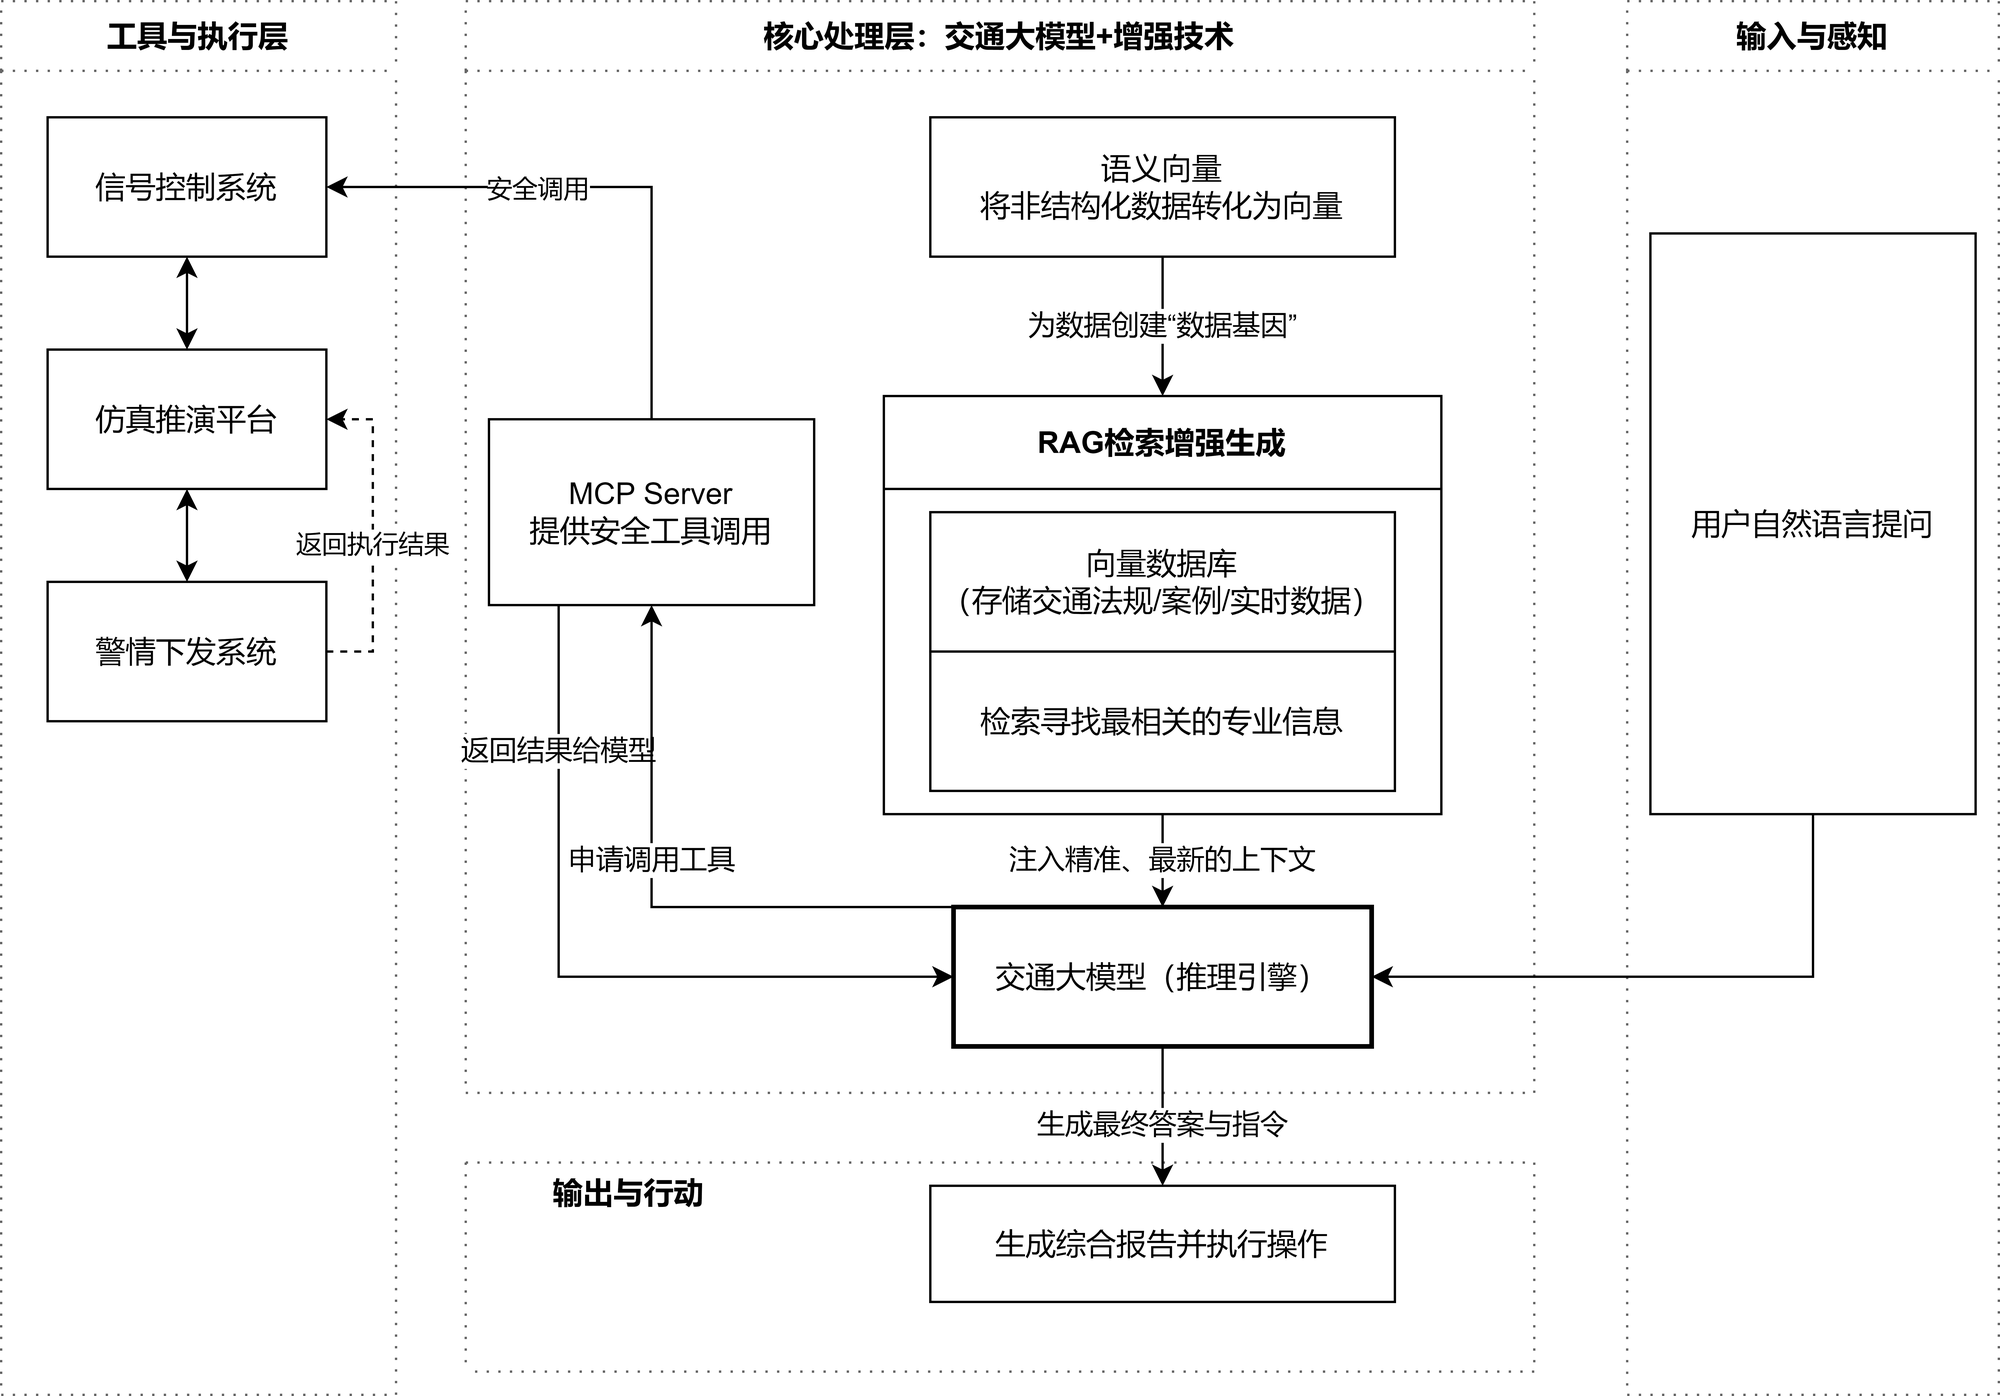
\includegraphics[width=0.8\textwidth]{figure/image1.png}
  \caption{交通智能体架构示意图}
  \label{fig:traffic-agent}
\end{figure}

就整体而言，智能体在代码、数学以及科学研究等各个方面已经取得了一些成熟的应用案例，在交通领域仍然处在起步阶段。现有的交通智能体研究大多使用通用的智能体架构，并没有很好地结合交通领域的时空预测模型来建立专门的解决方案。尤其是慢思考和快反应分工、多步推理和快速预测配合两方面的研究还存在着很大空间。本文工作就是在此方向上的一次尝试。